%!TeX root=../tese.tex
%("dica" para o editor de texto: este arquivo é parte de um documento maior)
% para saber mais: https://tex.stackexchange.com/q/78101/183146

% Vamos definir alguns comandos auxiliares para facilitar.

% "textbackslash" é muito comprido.
% \newcommand{\sla}{\textbackslash}

% Vamos escrever comandos (como "make" ou "itemize") com formatação especial.
% \newcommand{\cmd}[1]{\textsf{#1}}

% Idem para packages; aqui estamos usando a mesma formatação de \cmd,
% mas poderíamos escolher outra.
% \newcommand{\pkg}[1]{\textsf{#1}}

% A maioria dos comandos LaTeX começa com "\"; vamos criar um
% comando que já coloca essa barra e formata com "\cmd".
% \newcommand{\ltxcmd}[1]{\cmd{\sla{}#1}}

\chapter{Proposal and Preliminary Experiments}
\label{cap:proposal}

As discussed in the previous chapters, understanding how social networks
recommend content to users is central to the debate around the recent waves of
political polarization and radicalization that have been taking over many
developing and developed countries alike. There are many ways of exploring
recommender systems without examining their code, from simulating their behavior
after careful observation to directly collecting recommendation data, but most
of them allow us to examine only one perspective of the algorithm at work. This
means that studying a social network's recommendation technique has inherent
limitations.

Since the life and blood of almost all social media platforms revolve around
their recommendations, most of the algorithms currently employed by these
companies are trade secrets. They are also subject to constant experimentation
and tuning, which might render worthless any research performed before an update
to the algorithm, no matter how carefull the design of the study was. YouTube,
for example, currently has over 2 billion monthly logged-in users (which is more
people than any country in the planet), but it makes no significant effort to
clarify changes made to the algorithm or even whether they fulfill their
promisses of reducing user exposure to radicalizing content. With more than 500
hours of content being uploaded every minute, if 1\% of all videos can be
considered radicalizing and the algorithm can detect 99\% of them, that still
leaves over 25.000 hours of brand new extremist content free to spread on the
platform every year. YouTube claims only a small fraction of its content is
political in nature, but that doesn't mean it is not enough to spread across the
internet and help radicalize users the world over. It is also worth noting that
most of these platforms' efforts are concentrated in their parent countries
(usually the United States), so, even if they actually try and remove extreme
content, most of the non-English-speaking world would still not be impacted by
their policy changes.

Even with a quickly growing body of research, further studies are desperately
needed in order to shed more light into the inner workings of how recommendation
algorithms are used by social networks. Articles like the ones described in the
last chapter are of utter importance to this task, but generalist studies that
are able to capture dynamics common to all or most recommender systems are still
nonexistent.

This leads right into the goal of the present report. The dissertation to be
presented as a result of this program aims to make a tangible contribution to
the field of recommender systems, specifically how their design might (or might
not) foster confinement dynamics in the ``phase space'' of recommendations. If
the main hypothesis is confirmed, this could mean that recommendation algorithms
always create ``filter bubbles'', suggesting ever more engaging videos about a
certain topic of interest to a user, and possibly sending them on a
radicalization spiral if that topic is related to politics or other contentious
subjects.

\section{Experiments}
\label{sec:experiments}

Some preliminary experiments have already been conducted in order to gather some
evidence in favor or against the main hypothesis being tested. If these
experiments had failed, then there would be no reason to continue pursuing this
argumentative path. In total, fifteen different recommendation models were
trained and analyzed, with each visualization below representing one of these
models.

The goal of these experiments was trying to identify if even a simple
recommendation algorithm could demonstrate some sort of bias towards a subset of
the items being recommended. More specifically, given an algorithm that cannot
be influenced by users' personal preferences, would the resulting recommender
system favor some kind of item? Excluding user information is important because,
as demonstrated by \citet{stoica_algorithmic_2018}, users might have their own
biases and these would get transferred on to the model; the objective here is
understanding the algorithm by itself without external influences.

The chosen type of recommender system to be trained was, therefore, a
content-based recommender. In the real world this is an algorithm that is able
to identify similar items based on their metadata (description, tags, etc.) and
suggest the closest items to the one being purchased or viewed. A
straightforward way of building such an algorithm is creating a vector
representation of each item and then using a similarity metric to recommend the
items most similar to the one in question. The chosen similarity metric was
cosine similarity because of its simplicity, robustness, and ubiquity.

The main recommendation model (henceforth referred to as the ``vanilla'' model)
was trained with the MovieLens dataset \citep{harper_movielens_2015}. The
metadata for each movie was made up of its keywords, main cast, director, and
genres. The vector transformation was very simple, with each position
representing one of the words of the corpus, and each element indicating how
many times that word appeared in the metadata for that movie. When the
recommendation for a movie was requested, the algorithm measured the cosine
similarity between it and every other movie, returning the IDs belonging to
the top $k$ most similar vectors.

Once the model was ready, the analysis started: the algorithm was asked to
generate a list of the top $k = 10$ most similar movies to each movie; since
there were 30689 movies in the dataset, this created a list of $30689 \times 10$
movie IDs. After this computationally intensive calculation, the occurrence of
each ID was counted and ranked accordingly, namely, the movie ranked number 1
was to be the movie featured the most times in the set of all recommendations,
and so forth for every other rank. The result of this process can be seen in
Figure~\ref{fig:fig1:a}.

\begin{figure}
  \centering
  \begin{subfigure}{0.45\textwidth}
    \centering
    \includegraphics[width=\textwidth]{02_rec_vanilla}
    \caption{Rec. based on movie metadata.\label{fig:fig1:a}}
  \end{subfigure}
  \begin{subfigure}{0.45\textwidth}
    \centering
    \includegraphics[width=\textwidth]{16_rec_random}
    \caption{Random recommendations.\label{fig:fig1:b}}
  \end{subfigure}
  \caption{Vanilla recommendation model and control.\label{fig:fig1}}
\end{figure}

For comparison, Figure~\ref{fig:fig1:b} is the same visualization for the
trivial model (sampling $k$ movies at random when asked for a recommendation).
The number of times each movie appeared in the final list of all recommendations
averaged, evidently, $k$, with an appearance very similar to that of the CDF of
the normal distribution. The ``most recommended'' movie appeared 25 times in the
final list, while the ``least recommended'' movie did not appear at all.
However, the distribution of the vanilla model differs immensely: the movie
ranked number 1 appeared more than 2000 times in the final list, with an almost
exponential decrease in the number of appearances from then on.

In order to better understand this phenomenon, more models were trained and
analyzed. Since all visualizations present exactly the same quantities, obtained
in the exact same way, all of them can be compared.

\begin{figure}
  \centering
  \begin{subfigure}{0.3\textwidth}
    \centering
    \includegraphics[width=\textwidth]{03_rec_cutoff_med}
    \caption{Cutoff $n \leqslant 5$.\label{fig:fig2:a}}
  \end{subfigure}
  \begin{subfigure}{0.3\textwidth}
    \centering
    \includegraphics[width=\textwidth]{04_rec_cutoff_low}
    \caption{Cutoff $n \leqslant 2$.\label{fig:fig2:b}}
  \end{subfigure}
  \begin{subfigure}{0.3\textwidth}
    \centering
    \includegraphics[width=\textwidth]{05_rec_cutoff_high}
    \caption{Cutoff $n \leqslant 8$.\label{fig:fig2:c}}
  \end{subfigure}
  \caption{Vanilla model with cutoff point.\label{fig:fig2}}
\end{figure}

The first variation on the vanilla model that was experimented on was creating
cutoff points for words to be included in the vector representation of the
movies. Since most words appear only once (given that many are director and cast
names), the few movies whose metadata contained popular terms could have been
favored by the recommendation algorithm. Three cutoff points were created, and
the model was retrained with datasets that only contained words that appeared at
least twice, five times, and eight times. The results can be seen in
Figure~\ref{fig:fig2} and, aside from variations in the $y$-intercept, all plots
are qualitatively very similar to Figure~\ref{fig:fig1:a}.

\begin{figure}
  \centering
  \begin{subfigure}{0.3\textwidth}
    \centering
    \includegraphics[width=\textwidth]{06_rec_cosine}
    \caption{Cosine distance.\label{fig:fig3:a}}
  \end{subfigure}
  \begin{subfigure}{0.3\textwidth}
    \centering
    \includegraphics[width=\textwidth]{07_rec_euclidean}
    \caption{Euclidean distance.\label{fig:fig3:b}}
  \end{subfigure}
  \begin{subfigure}{0.3\textwidth}
    \centering
    \includegraphics[width=\textwidth]{08_rec_manhattan}
    \caption{Manhattan distance.\label{fig:fig3:c}}
  \end{subfigure}
  \caption{Using distances instead of cosine similarity.\label{fig:fig3}}
\end{figure}

The second validation experiment involved using distance metrics instead of
cosine similarity. The goal here was verifying whether other metrics could
do a better job at not creating a subset of movies that ended up exponentially
more recommended that the rest. As attested by Figure~\ref{fig:fig3}, this was
not the case. No other similarity metrics were used because cosine seems to be
the most popular one used in simple recommender systems. More experiments have
still to be conducted on this front, specially comparing what IDs belong to
the group of top-recommended movies for each metric and if there is intersection
between them.

\begin{figure}
  \centering
  \begin{subfigure}{0.3\textwidth}
    \centering
    \includegraphics[width=\textwidth]{11_rec_p}
    \caption{$P(w) = P(V_w)$.\label{fig:fig4:a}}
  \end{subfigure}
  \begin{subfigure}{0.3\textwidth}
    \centering
    \includegraphics[width=\textwidth]{12_rec_p10}
    \caption{$P(w) = 10 \times P(V_w)$.\label{fig:fig4:b}}
  \end{subfigure}
  \begin{subfigure}{0.3\textwidth}
    \centering
    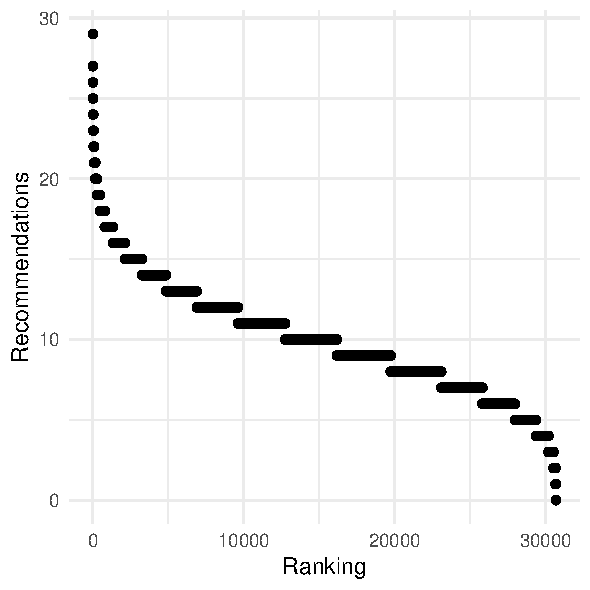
\includegraphics[width=\textwidth]{13_rec_p100}
    \caption{$P(w) = 100 \times P(V_w)$.\label{fig:fig4:c}}
  \end{subfigure}
  \caption{Random sample of words from metadata.\label{fig:fig4}}
\end{figure}

At this point it is safe to say that the exponential decay in recommendation
frequencies is not spurious and must have a clear cause. A hypothesis that was
later mostly confirmed involved the average number of non-zero elements in the
vector representation of the movies: the sparser the vectors, the higher the
odds of the recommendation curve displaying a steep left-hand side.
Figure~\ref{fig:fig4} displays the curves of three different models trained from
random data; for each, the propability of an element being non-zero in the
vector representation of a movie was the average probability that an arbitrary
element of the MovieLens dataset was non-zero (times 1, 10, and 100). This was
equivalent to creating random metadata for the movies where the probability of a
word occurring was approximately $1.54 \times 10^{-4}$, $1.54 \times 10^{-3}$,
and $1.54 \times 10^{-2}$ respectively. The results support the aforementioned
hypothesis.

\begin{figure}
  \centering
  \begin{subfigure}{0.45\textwidth}
    \centering
    \includegraphics[width=\textwidth]{09_rec_artificial_movie}
    \caption{Artificial movie.\label{fig:fig5:a}}
  \end{subfigure}
  \begin{subfigure}{0.45\textwidth}
    \centering
    \includegraphics[width=\textwidth]{14_rec_long}
    \caption{Long and narrow.\label{fig:fig5:b}}
  \end{subfigure}
  \caption{Sanity checks.\label{fig:fig5}}
\end{figure}

Figure~\ref{fig:fig5} showcases two sanity checks. Figure~\ref{fig:fig5:a} was a
model trained with the vanilla dataset, but with the addition of an artificial
movie created as a combination of the metadata from other movies favored by the
recommendation algorithm. As expected, this movie also featured in the
top-recommended subset. Figure~\ref{fig:fig5:b} comes from a model trained on
random data generated in a similar fashion to the model in
Figure~\ref{fig:fig4:a}, except each vector could only have 15,000 elements
instead of 55,681 as with the vanilla model (which is why it is called ``long
and narrow''). The patter observed before persisted.

\begin{figure}
  \centering
  \begin{subfigure}{0.45\textwidth}
    \centering
    \includegraphics[width=\textwidth]{10_rec_books}
    \caption{Book dataset.\label{fig:fig6:a}}
  \end{subfigure}
  \begin{subfigure}{0.45\textwidth}
    \centering
    \includegraphics[width=\textwidth]{15_rec_mimic}
    \caption{Simulation of vanilla.\label{fig:fig6:b}}
  \end{subfigure}
  \caption{Confirmation of hypothesis.\label{fig:fig6}}
\end{figure}

The last two models were considered the confirmations of the hypothesis that
(at least for this kind of recommendation systems) a subset of items was always
exponentially more recommended than the rest as long as the data was sparse.
Figure~\ref{fig:fig6:a} represents the same recommendation algorithm applied to
another dataset, the Book-Crossing Dataset. Figure~\ref{fig:fig6:b} contains the
results of the model applied to another random dataset, this time with the
probability of each element being non-zero respecting the marginal distributions
of the vanilla dataset. Again, the exponential decay pattern persisted, only
slightly less pronounced in the Book-Crossing case.

\section{Further Experiments and Schedule}
\label{sec:schedule}

Lorem ipsum.
